\documentclass[hidelinks,12pt]{article}
\usepackage[utf8]{inputenc}
\usepackage[T1]{fontenc}

%% A SUPPRIMER A LA FIN
\usepackage[french]{babel}

\usepackage{times}
\usepackage{hyperref}
\usepackage{graphicx}
\usepackage{caption,graphicx,enumitem}
\usepackage{amsmath}
%\usepackage{titlesec}

%\setcounter{secnumdepth}{4}


\begin{document}

\title{Study of a surrogate model for shallow water equations}
\author{Bastien Nony, Alban Gossard\\
Institut National des Sciences Appliquées,\\
Toulouse,\\
\href{mailto:nony@etud.insa-toulouse.fr}{   \texttt{nony@etud.insa-toulouse.fr}}\\
\href{mailto:gossard@etud.insa-toulouse.fr}{   \texttt{gossard@etud.insa-toulouse.fr}}}
\date{\today}

\maketitle

\begin{abstract}
In this work we study surrogates problems for different types of modelling problem. The objective is to provide fast calculation for undetermined values. Beginning from physical equations such as Saint-Venant's, we add statistical formulas to determine the variability of the system. This study registers in the frame of geostatistics.
\end{abstract}

\newpage

\tableofcontents

\section{Introduction}

The resources management and the flood forecast requires a solid anticipation which relies onto solid hydraulic models. The numerical breakthroughs allowed huge progress in computational efficiency.

The shallow water equations (SWE) derived from the Navier Stokes for free surface flows proved their efficiency for flood problems in open channels. Regardless, any prediction requires a good knowledge of certain initial values : physical coefficient such as friction and initial flow rate, river bathymetry and boundary conditions. These values vary over time. Because of a lack of knowledge we must assume the input parameters are subject to hazard. Then, variability exists and can come from the nature of the numerical model but also from the environment such as the weather or the season. With this idea we proceed to uncertainty quantification and study output errors and the influence of each input parameter which could limit the effectiveness of the forecast. The objective of uncertainty quantification is to study and to classify the different sources of variability to limit the errors in output. The aim is to better build numerical models to make them less fragile in front of uncertainties, to propose better estimates for reduced computation time.

Indeed, physico-numerical models are long to compute. To avoid this problem we generate a surrogate model given a few number of values. The idea is the following : the original based on physical equations give the best approximation of reality we can expect. We use this model to determine a few amount of points and given these results we interpolate them to have a full model on our study area. 
We consider certain input parameters. As we will see in the following, in the "Chanel Flow" model we consider two input parameters : $Q$ which is the initial flow and $K_s$ the Strickler's coefficient. Because the parameters can vary in time, we model them using random variables. The calibrations are given by experts. 
If the model's computation is too time-consuming, we prefer to evaluate a surrogate model cheaper in time-cost. In our example we will choose two different types of models : kriging and polynomial chaos. Because surrogate models are just an approximation of the physical ones, we have to evaluate uncertainty and the influence of each parameters on the output values.

We will introduce briefly the different tools used in our projects. The first tests will be set on the "Chanel flow" model and the Mickalevitch function. In the last part we will test the efficiency of a surrogate model based on values coming from the Garonne's river, computed using MASCARET-TELEMACS.


\section{Objectives}
\section{Key notions}


\section{Sources d’incertitude}

%ATTENTION : paragraphes à approfondir car une seule source (Fajraoui_noura2014)


\subsection{Incertitude structurelle }

Incertitude liée au modèle mathématique, approximation de la réalité. Les hypothèses simplifient les phénomènes physiques et/ou ne les prennent pas tous en considération. Dans notre cas les équations de Saint Venant sont des équations 1D en eau peu profonde.

\subsection{Incertitude numérique}


Imprécisions liées aux approximations numériques qui s’accumulent dans les calculs. les solutions ne sont pas forcément analytiques et chaque étape de calcul peut conduire à une approximation qui s’additionne aux précédentes, par exemple enchaînement d’erreurs d’arrondi. L’incertitude numérique concerne aussi l’erreur de discrétisation spatiale obtenue lors des relevés physiques effectués par les spécialistes sur le terrain.

\subsection{Incertitude paramétrique}

Incertitude obtenue par la variabilité des paramètres d’entrée ou du manque d’information ou du biais d’un échantillon de départ. Un test statistique effectué sur un échantillon non représentatif peut mener à des résultats complètement biaisés.




\section{Surrogate Models}

Calculating all values is impossible for computing time reasons. Suppose we wanted to determine the distribution of coal density over each square meter of the Lorraine region, the task would be long and tedious. Each statement would cost time and money. Instead of taking too many measurements on each square meter, we propose to reduce the number of measurements and then interpolate the data over the entire space map. This problem gave rise to the so-called kriging technique.

A first idea would be to interpolate deterministically by linear, polynomial interpolation. This method raises several problems. It will be impossible by mathematical formalism to quantify uncertainty. Indeed, the deterministic variables do not make it possible to estimate potential/unforeseeable variations. For this reason, an alternative proposes a stochastic interpolation.

In this paper we use different methods for computing surrogate models. In this part we present some of their main characteristics.


\subsubsection{Kriging}

Kriging consists in creating a linear estimator from measurements already made before. Using the physical model, $n$ output values $(Y_1,\ldots,Y_n)$ are determined for inputs distributed over our study set. 

The estimator noted $\hat{Y}$ then : $\hat{Y}=\sum_{i=1}^{n}\lambda_i Y_i$ where $\lambda_i$ are scalar values associated to each $Y_i$.

This estimator has several advantages. It is the best linear unbiased predictor. This means it minimizes the variance of errors $Var[\hat{Y}-Y]^2$, it is a linear combination of the measures $Y_i$ and it is unbiased $E[\hat{Y}-Y]=0$.
\begin{enumerate}
\item Also, $\hat{Y}$ admits the perfect values at the $Y_i$ measures.
\item To infinity the points do not bring any more information on the result.
\item The estimator is a convex combinaison of the measures : $\sum_{i=1}^{n}\lambda_i=1$
\item If there are many values in a given region then the weights are low. This is because each point has a greater impact on areas that is close to it and less on remote areas where information is shared between a lot of data points.
\item In areas where there is little data, kriging reflects an estimate of the average. Indeed the values influence in a roughly equivalent way on the very distant points.
\end{enumerate}

\subsubsection{Ordinary kriging solving system}
We place ourselves in the framework of a stationary random function. Thus:

$$E[Y_i]=E[Y_j]=\mu, \forall i,j$$

and $$Cov(X_i,X_{i+h})=\gamma(h), \forall i$$

The fact that our kriging estimator is of minimal variance and is unbiased at points $Y_i$ gives us:

$$E[Y_0-Y_i]=0$$
So, $$\sum_{i=0}^{n}\lambda_iE[Y_i]=E[Y_i]$$
Then, $$\mu \sum_{i=1}^{n}\lambda_i = \mu$$

If we don't know the value of $\mu$, we need to have $$\sum_{i=1}^{n}\lambda_i=1$$

The second condition on the minimal variance gives : 
$$ (\lambda_1,\ldots,\lambda_n)= \arg\min_{\sum \lambda_i=1} Var(\hat{Y}_0-Y_0)$$

We solve this convex optimization problem using the following lagrangian :

$$L(\alpha)=Var(\hat{Y}_0-Y_0)+\alpha(\sum_{i=0}^{n}\lambda_i-1)$$

This brings us to the following result :

$$\forall i \in {1,\ldots, n}, \sum_{i=1}^{n}\lambda_j Cov(Y_i,Y_j)+ \alpha = Cov(Y_0,Y_i)$$

Using matrices we need to solve the following system :

$$
\begin{bmatrix}
\gamma_{11}& \cdots  & K_{1j} & 1\\ \vdots & \ddots & \vdots & \vdots \\ K_{i1} & \cdots  & K_{nn} & 1 \\ 1 & \cdots & 1 & 0 
\end{bmatrix} 
\begin{bmatrix}
\lambda_1 \\ \vdots \\ \lambda_n \\ - \mu 
\end{bmatrix} = 
\begin{bmatrix} K_{10} \\ \vdots \\ K_{n0} \\ 1
\end{bmatrix}.$$

where $K_{ij}=Cov(Y_i,Y_j)$

Travail à faire ensuite : finir partie krigeage en ajoutant la variance obtenue. Peut-être donner un estimateur du variogramme. 



Introduisons quelques outils statistiques :

\subsection{Variogramme}





\subsection{Interpolation par krigeage}

Cette méthode est probablement la plus évidente relativement au formalisme mathématique. Il s'agit d'une estimation linéaire où chaque estimation se fera linéairement en fonction de valeurs exactes mesurées au environs et associées à des poids particuliers.

Ainsi, la procédure est la suivante :

(1) On délimite notre zone d'étude en intervalles de paramétrage.

(2) On mesure, calcule à partir d'un modèle physique de départs un certain nombre de données idéales ($X_1,\ldots,X_n$)

(3) Pour un certain point donné dans notre espace délimité on trouve l'estimateur associé en calculant la matrice de poids correspondante.
(4) notre estimateur en ce point vaut donc la somme des valeurs idéales * leur poids estimé correspondant

Mathématiquement cela donne :

(1) pour un krigeage simple




(2) Pour un krigeage ordinaire

Cette approche apporte plusieurs avantages :


Tout d'abord il est possible de quantifier la variance de notre estimation par le biais de la variance du krigeage :



Les poids de krigeage adoptent des caractéristiques logiques :

(1)A l'infini les points n'apportent plus d'information sur le résultat

(2) Si le nombre de valeurs dans une région donnée est grand alors les poids sont très faibles. Cela s'explique par le fait que chaque point influe davantage sur les zones qui lui sont très proches et moins sur les zones lointaines où l'information se partage entre beaucoup de données.

(3) Dans les régions où il y a peu de données, le krigeage reflète une estimation de la moyenne.

\section{Méthode de quadrature}
\section{Interpolation par polynomes du chaos}


Comment choisir les points de référence? Méthode quasi aléatoires
\section{Méthodes d’échantillonage}

Dans ce paragraphe nous traitons la problématique de l’échantillonnage de l’espace de départ. L’échantillon de départ est limité à N données. Comment les choisir de manière optimale? 

Une première idée consiste à les quadriller de manière régulière notre espace de départ. Pour des raisons de périodicité et de régularité cette méthode peut conduire à l’obtention d’un échantillon non représentatif de la population de départ. Par exemple nous voulons modéliser la fonction sinus sur l’intervalle $[0,2k\pi ]$. Si les relevés sont effectués régulièrement tous les $2i\pi$ alors on pourra penser que la fonction sinus est constante égale à 1. 

D’autres approches permettent de limiter ce risque. Nous allons tout d’abord voir les méthodes de Monte-Carlo puis des méthodes quasi-aléatoires comme la méthode de séquencement de Halton.

\subsection{Méthodes de Monte-Carlo}

Les échantillons ont tendance à se regrouper autour de la région à forte densité


\subsection{Latin Hypercube Sampling}

Meilleur couverture du sampling

\subsection{Séquence de halton}




\section{Study of 1D model}
\subsection{Presentation}
\subsection{Theoretical tools}
\subsection{Surrogate model analysis}
\subsubsection{First example : Ishigami}
\subsubsection{Garonne Model }

\paragraph{Surrogate method : kriging}
\hspace{1cm}

We compute different surrogate using different initial sample size. These surrogates were computed using a least square strategy. Figure \ref{influence_init_size_method_surrogate_kriging} gives the simulations results for the surrogate. One can observe that we obtain almost the same resultats as the initial sample size is greater than 10. As we will explain in part \ref{}, the results are quite precise but we have no information about the standard deviation of this new model and its sensibility to the parameters. Computing a surrogate with a greater number of points is fundamental to get a quantification of the error.

\begin{figure}
  \centering
  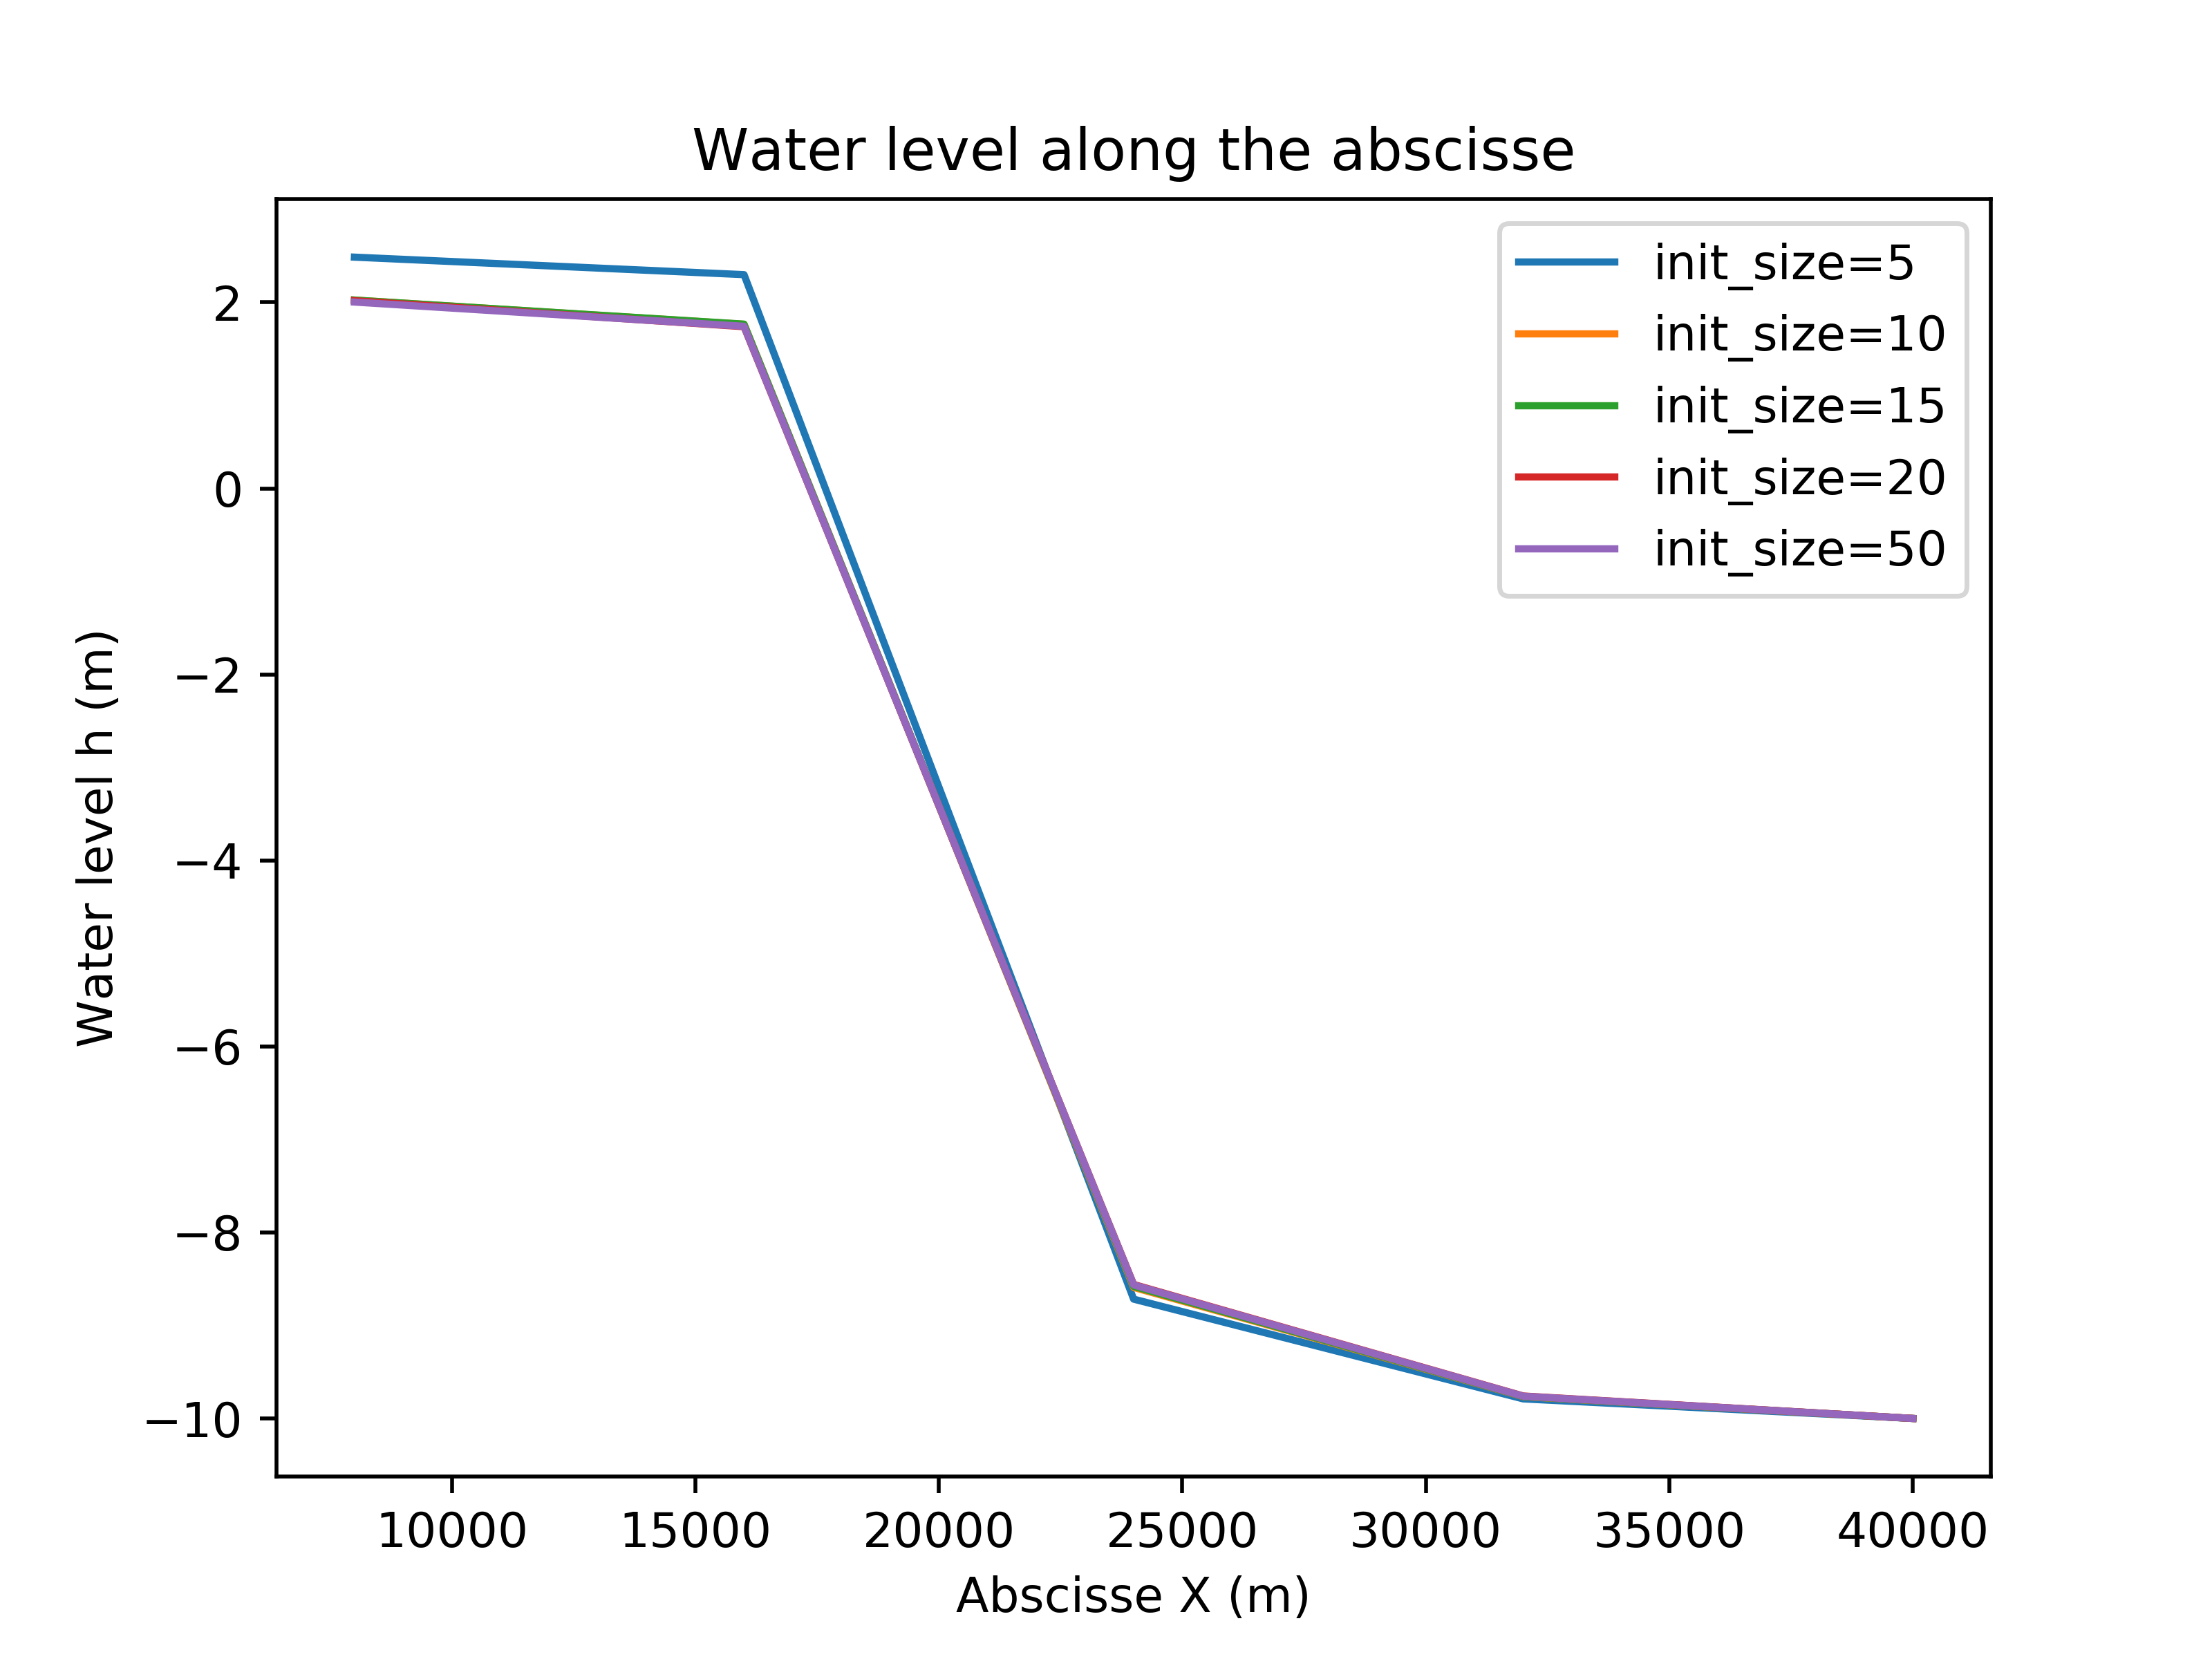
\includegraphics[width=0.8\textwidth]{images/influence_init_size_method_surrogate_kriging.png}
  \caption{Water level along the abscisse for simulations with different initial sample size using kriging method for surrogate computing.}
  	\label{influence_init_size_method_surrogate_kriging}
\end{figure}

\paragraph{Surrogate method : pc}
\hspace{1cm}

\begin{figure}
  \centering
  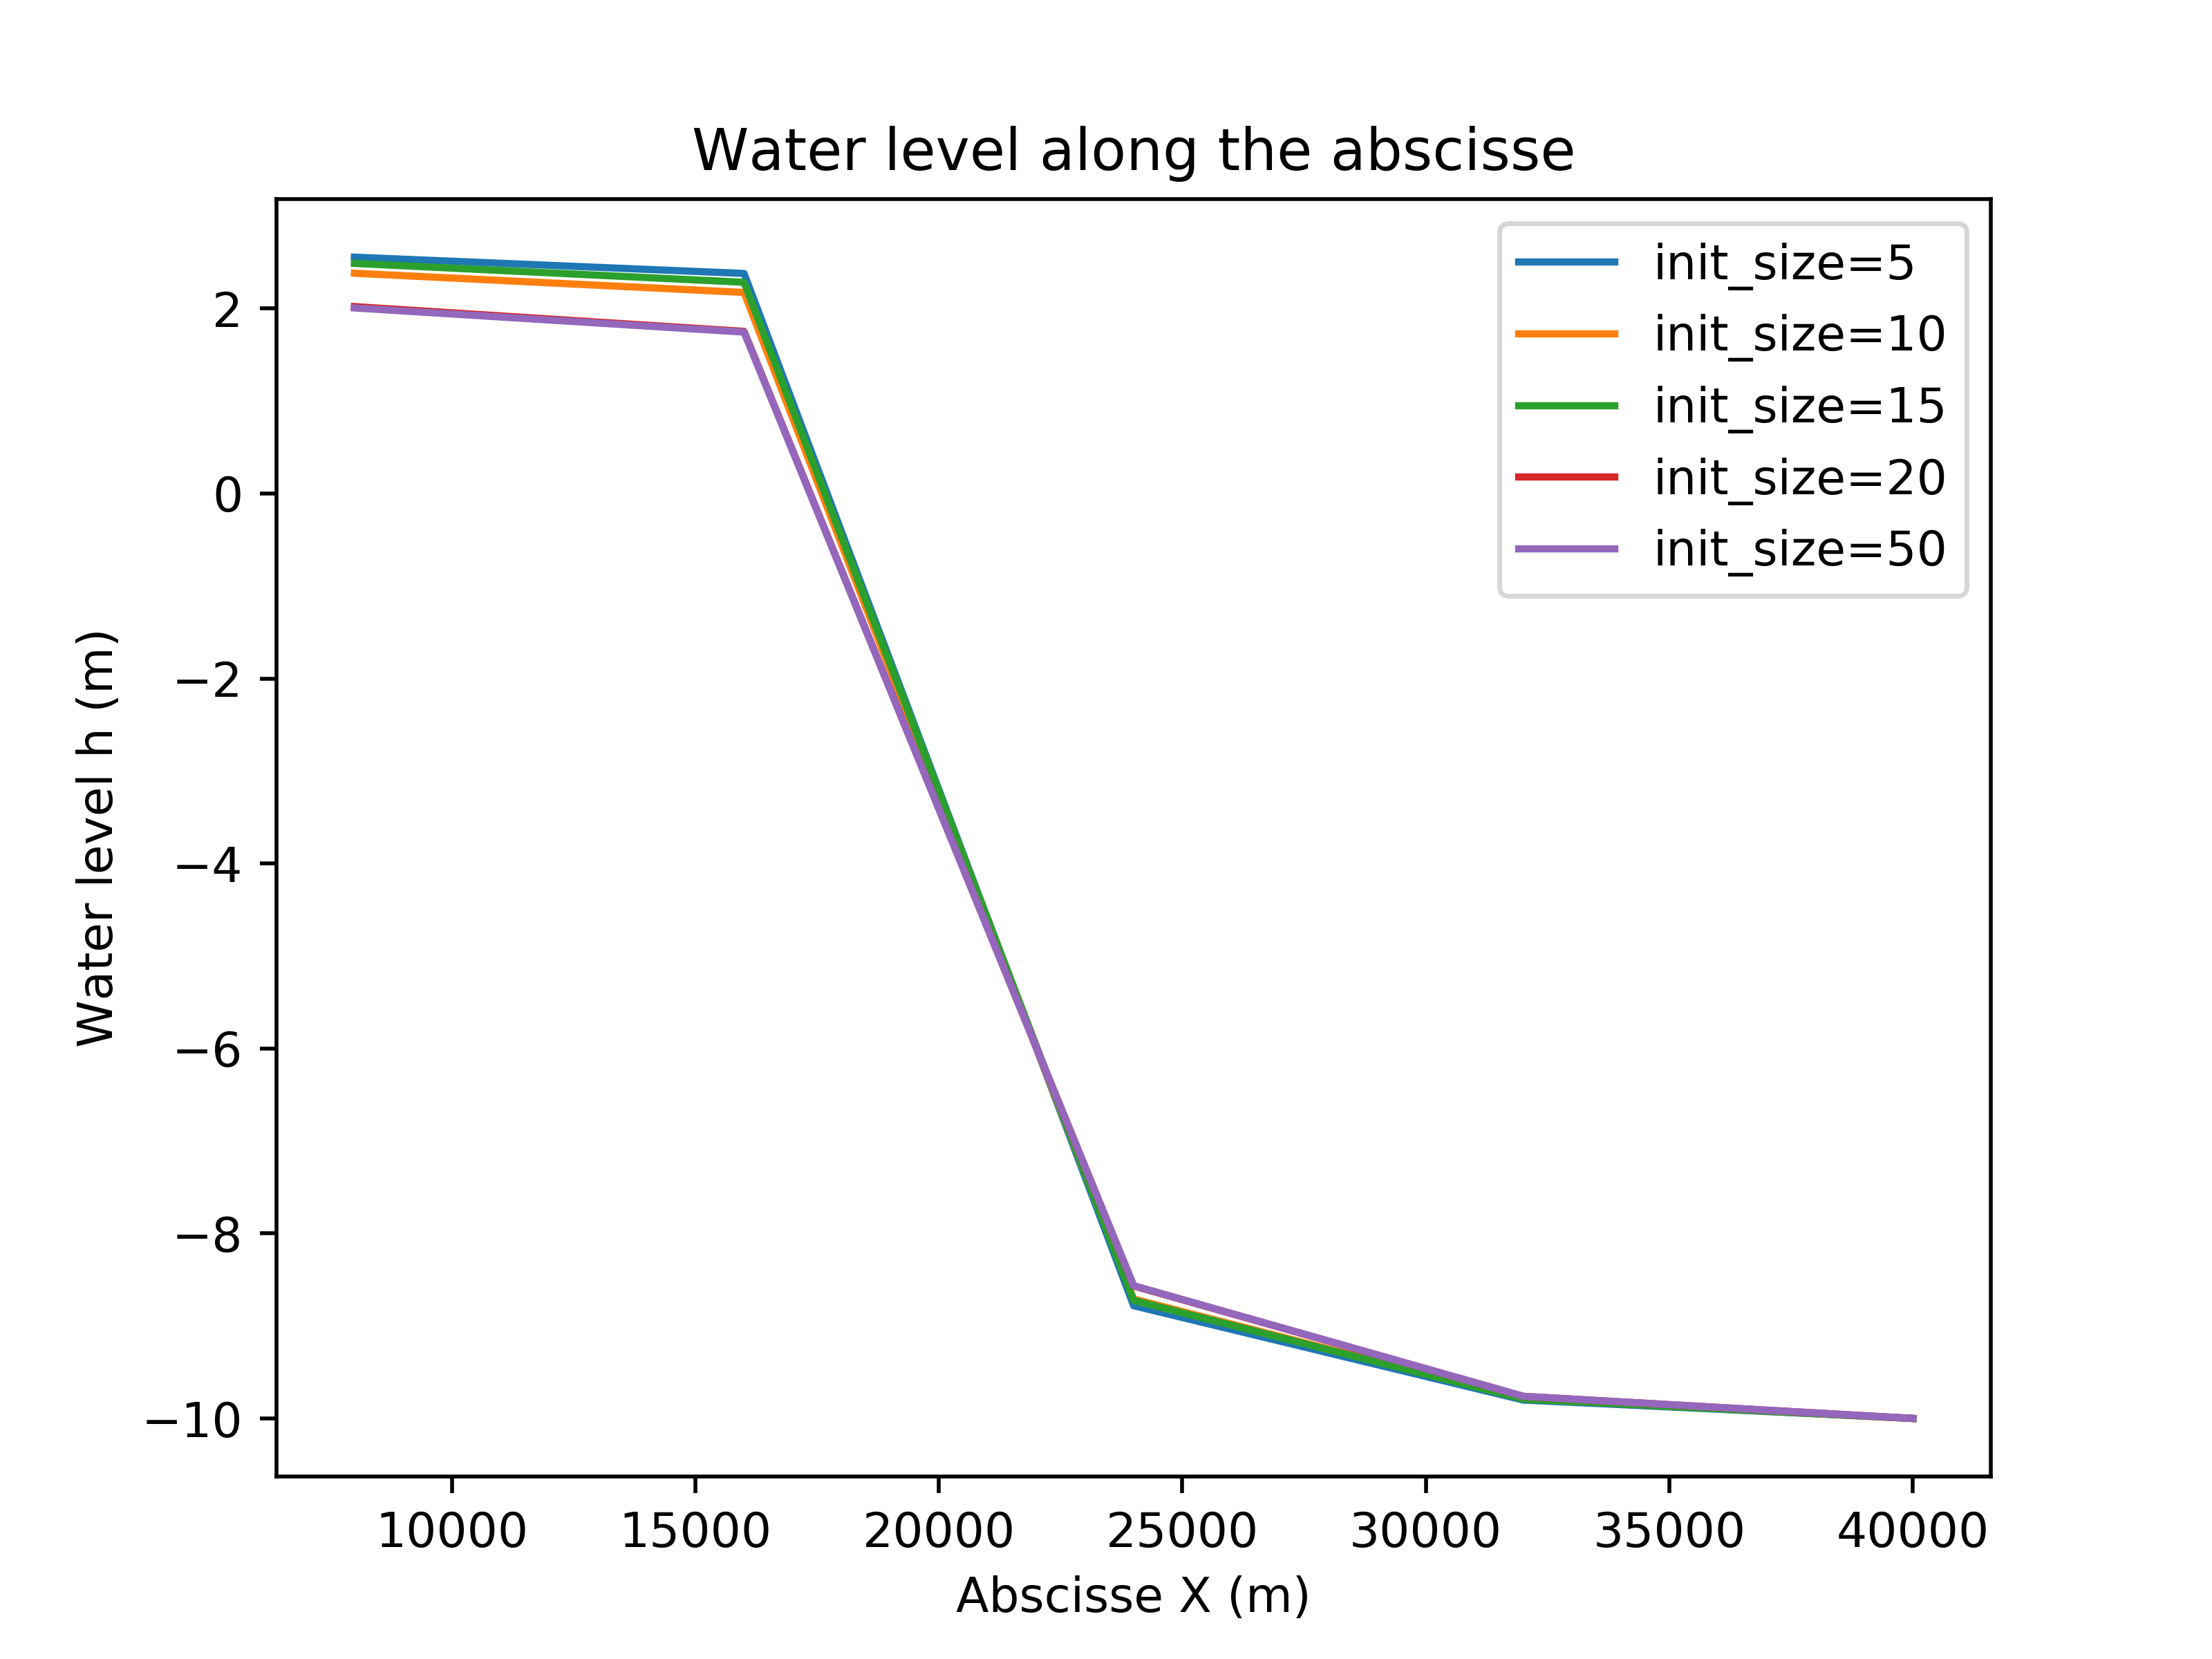
\includegraphics[width=0.8\textwidth]{images/influence_init_size_method_surrogate_pc.png}
  \caption{Water level along the abscisse for simulations with different initial sample size using pc method for surrogate computing.}
  	\label{influence_init_size_method_surrogate_pc}
\end{figure}

\begin{figure}
  \centering
  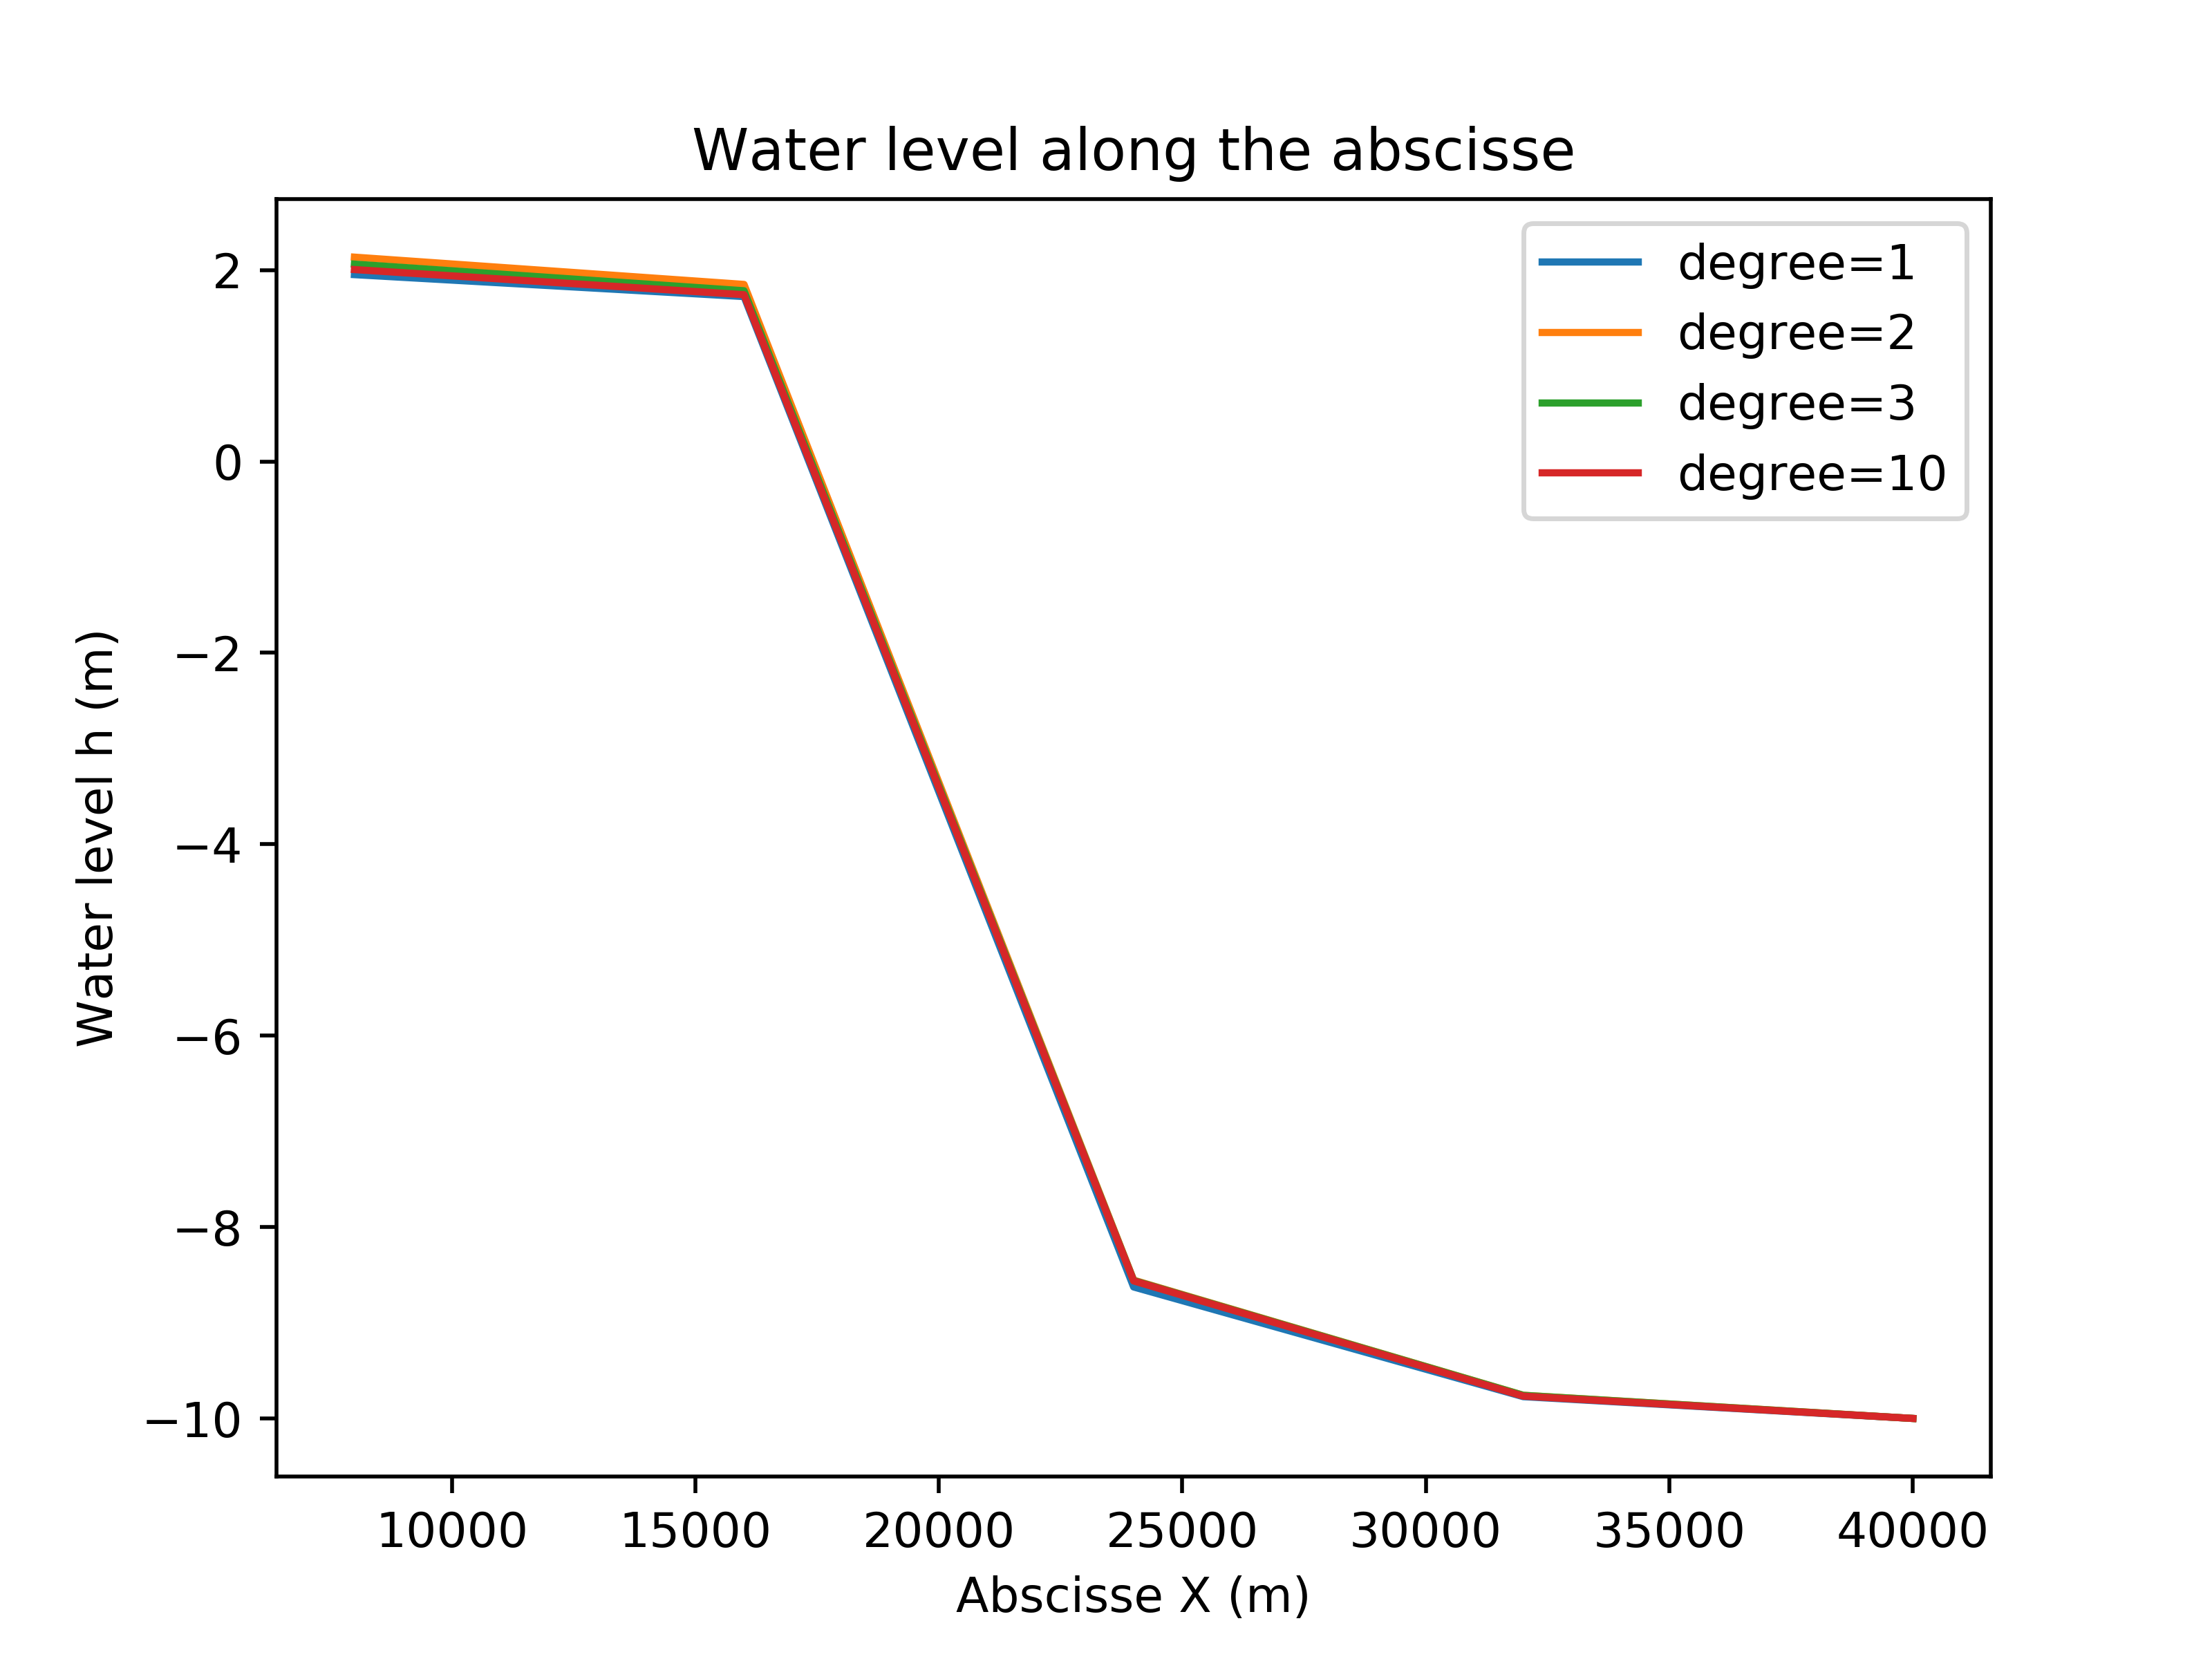
\includegraphics[width=0.8\textwidth]{images/influence_degree_method_surrogate_pc.png}
  \caption{Water level along the abscisse for simulations with different maximum pc degree.}
  	\label{influence_degree_method_surrogate_pc}
\end{figure}

\paragraph{Q2 study}
\hspace{1cm}

\begin{table}
\begin{tabular}{|c|c|}
  \hline
  Max pc degree & Q2 value \\
  \hline
  1 & 0.77805266\\
  2 & 0.95102133\\
  3 & 0.99238156\\
  4 & 0.99782457\\
  5 & 0.99813309\\
  \hline
\end{tabular}
\caption{Q2 value for different maximum pc degree using pc method for surrogate computing.}
\label{influence_degree_method_surrogate_pc_Q2}
\end{table}

\subparagraph{Distributions}
\hspace{1cm}

\begin{figure}
  \centering
  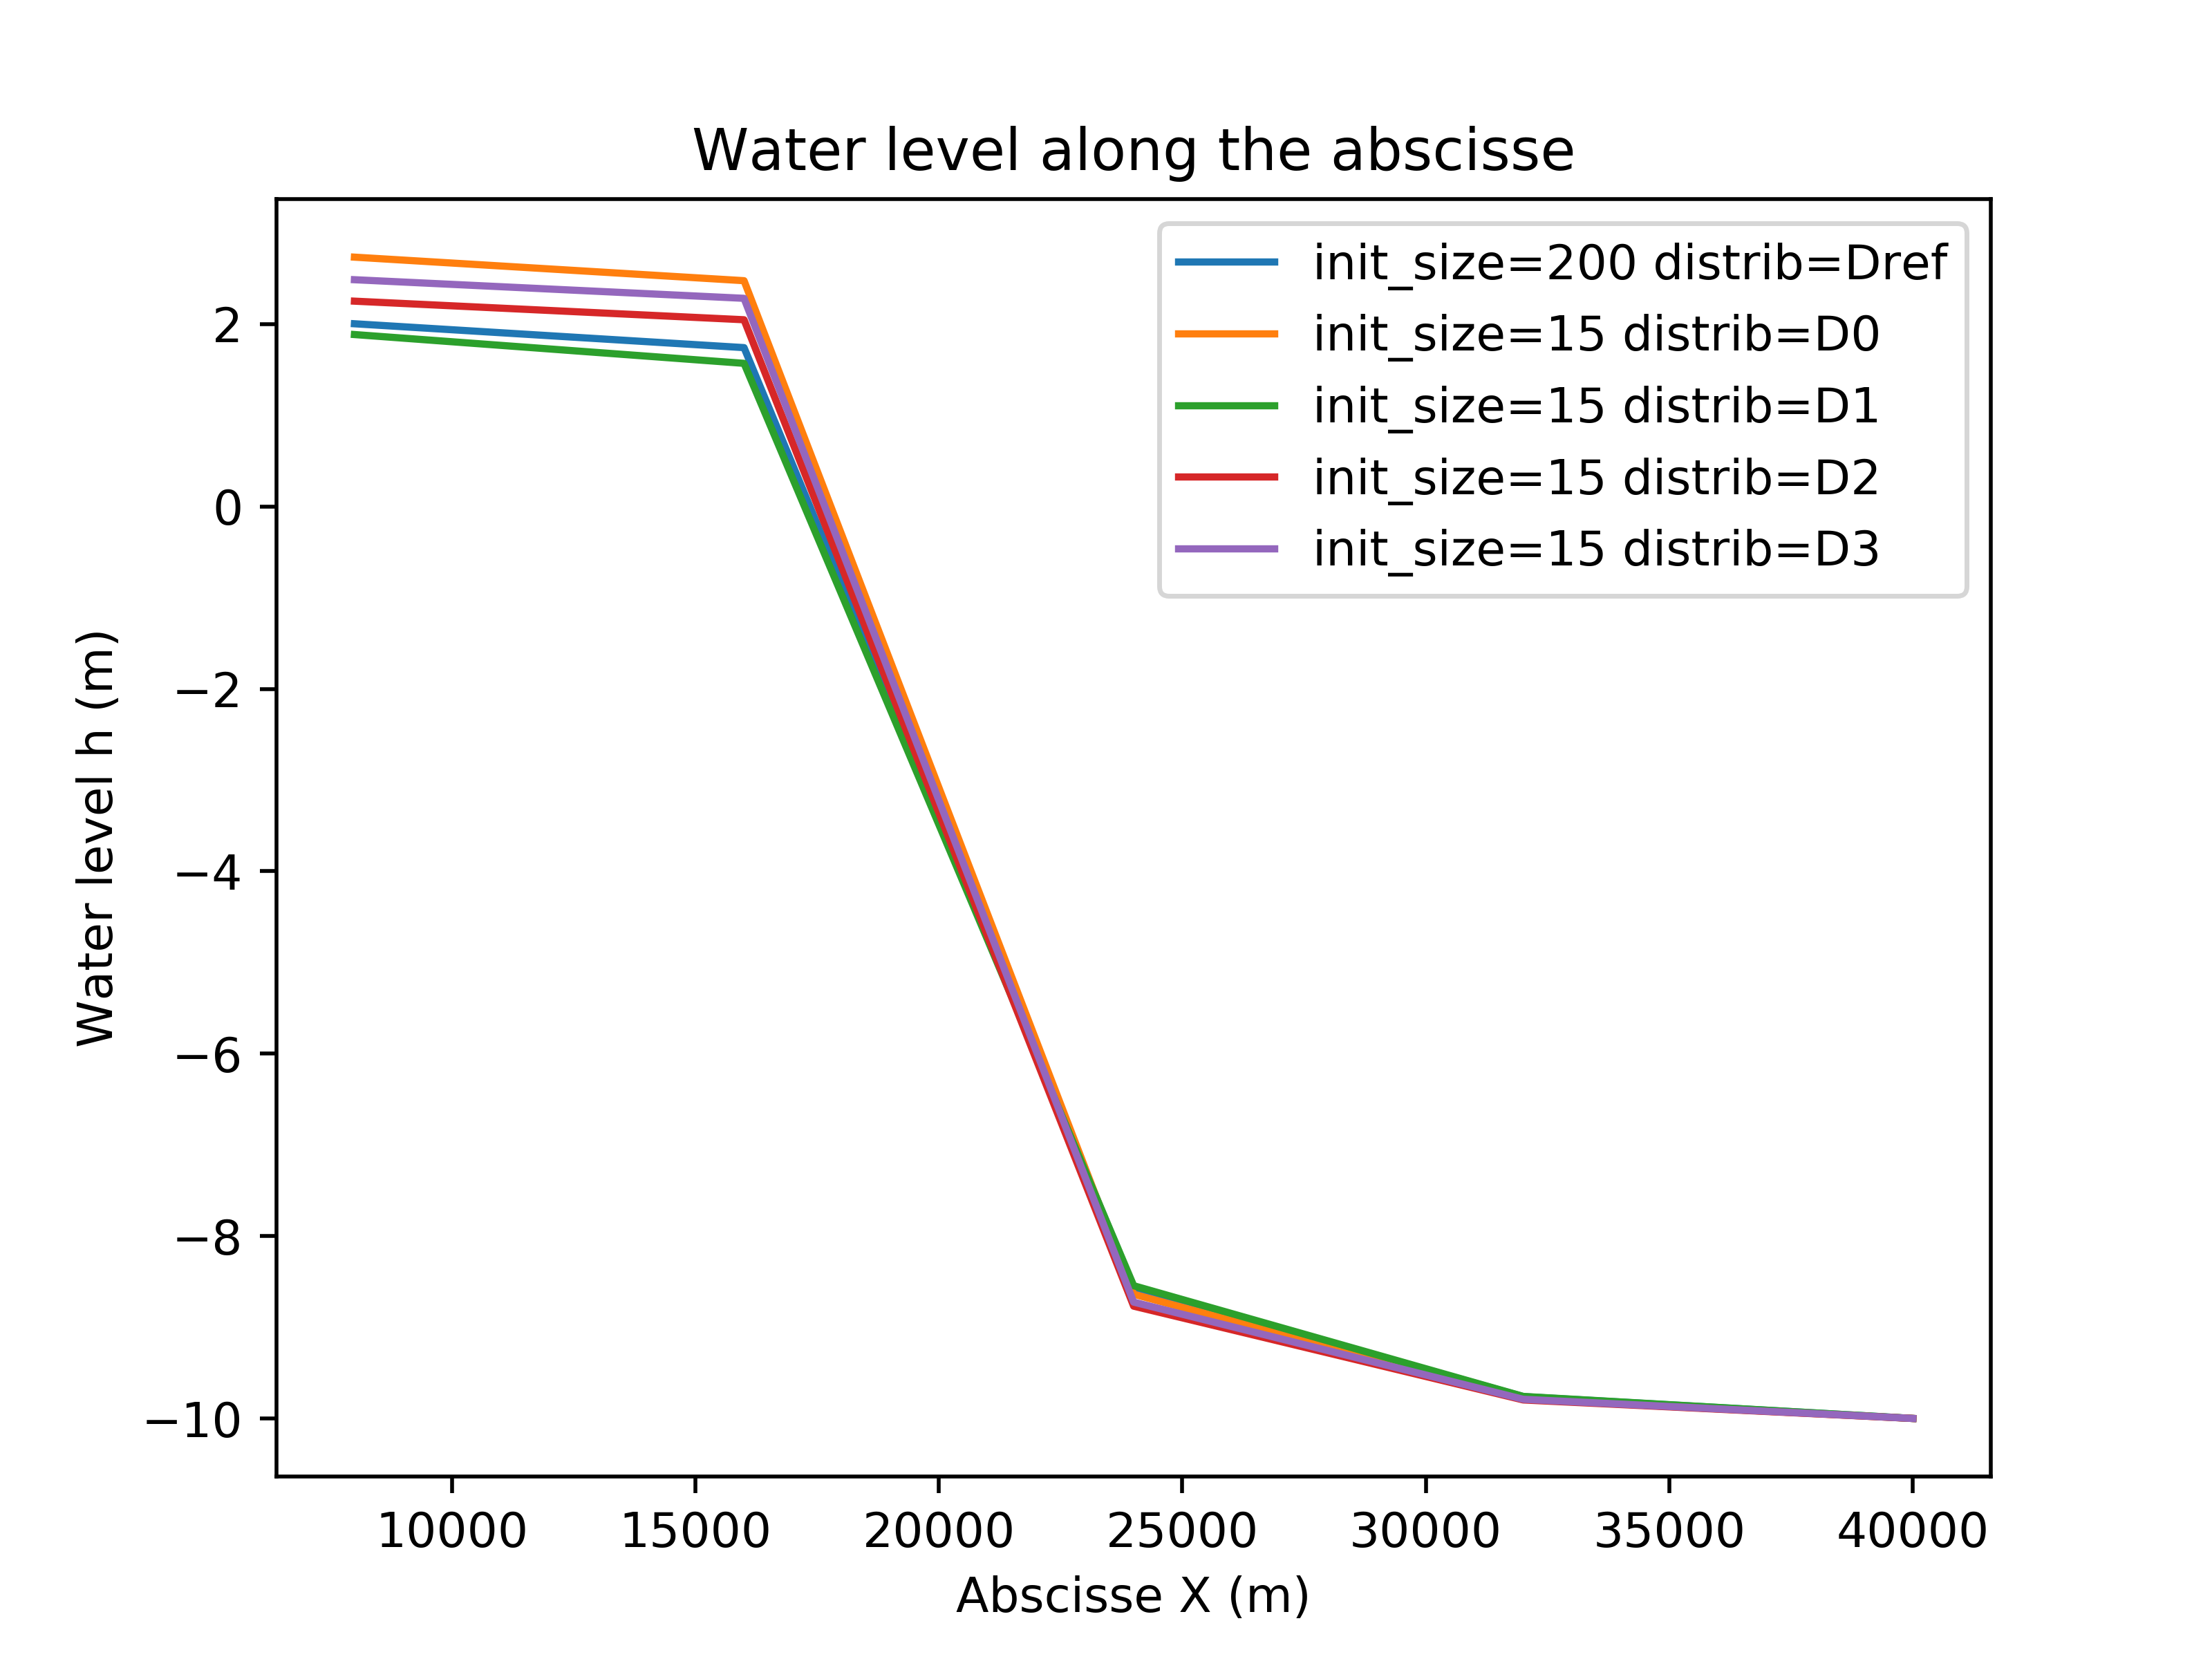
\includegraphics[width=0.8\textwidth]{images/influence_distributions_least_square.png}
  \captionsetup{singlelinecheck=off}
  \caption[]{Water level along the abscisse for simulations with different distributions for $Q$ and $K_s$ using least square strategy for surrogate computing. Distributions are the following : \begin{itemize}
  \item $D_{ref}$ : $K_s\sim BetaMuSigma(37.5, 5, 15, 60)$, $Q\sim BetaMuSigma(4035, 400, 2500, 6000)$
  \item $D_0$ : $K_s\sim Uniform(15, 60)$, $Q\sim Uniform(2500, 6000)$
  \item $D_1$ : $K_s\sim Uniform(15, 60)$, $Q\sim BetaMuSigma(4035, 400, 2500, 6000)$
  \item $D_2$ : $K_s\sim BetaMuSigma(37.5, 5, 15, 60)$, $Q\sim Uniform(2500, 6000.)$
  \item $D_3$ : $K_s\sim BetaMuSigma(37.5, 5, 15, 60)$, $Q\sim BetaMuSigma(4035, 400, 2500, 6000)$
  \end{itemize}}
  	\label{influence_distributions_least_square}
\end{figure}

One can consider that the $D_{ref}$ distribution is a good approximation of real $Q$ and $K_s$ values, meaning that we can compare different distributions with an initial sample size small to $D_{ref}$ distribution (which is computed with a high initial sample size). Figure \ref{influence_distributions_least_square} gives water level along abscisse for different sampling distributions on $Q$ and $K_s$. The distribution $D_1$ is the closest one to $D_{ref}$ suggesting we should sample the space $(Q,K_s)$ using a uniform distribution on $K_s$ and a normal one on $Q$.

\subsubsection{Michalewicz example}





%\section{Annex}

%\subsection{Polynomial Chaos} ?????




\end{document}
